\documentclass{article}

\usepackage{Engineering}
\usepackage{multicol}
\usepackage{tcolorbox}
\usepackage{titlesec}
\usepackage{titling}
\usepackage{etoolbox}
\usepackage{tabularx}

% === METADATA ===
\pdftitle{EFPLab1 Cheatsheet}

% === HEADER/FOOTER ===
\usepackage{fancyhdr}
\pagestyle{fancy}
\fancyhf{}
\lhead{Matteo Frongillo}
\chead{EFPLab1 Cheat Sheet}
\rhead{\thepage}

% === CUSTOM BOX COMMANDS ===
\definecolor{BoxBG}{HTML}{F0F8FF}
\definecolor{BoxBorder}{HTML}{3B83BD}

\newtcolorbox{theorybox}[1]{
  colback=BoxBG,
  colframe=BoxBorder,
  fonttitle=\bfseries,
  left=1mm,right=1mm,top=1mm,bottom=1mm,
  boxrule=0.8pt,
  arc=1.5mm,
  title={\begingroup\intheoryboxtitletrue #1\endgroup\intheoryboxtitlefalse}
}

\newtcolorbox{examplebox}[1]{
  colback=gray!10!white,
  colframe=gray!80!black,
  coltitle=white,
  fonttitle=\bfseries,
  left=1mm,right=1mm,top=1mm,bottom=1mm,
  boxrule=0.8pt,
  arc=1.5mm,
  title={#1}
}

\newtcolorbox{formula}[1]{
  colback=green!10!white,
  colframe=green!50!black,
  fonttitle=\bfseries,
  left=1mm,right=1mm,top=1mm,bottom=1mm,
  boxrule=0.8pt,
  arc=1.5mm,
  title={#1}
}

% === SECTION TITLE FORMATTING ===
\newif\ifintheoryboxtitle
\intheoryboxtitlefalse

\titleformat{\section}
  {\ifintheoryboxtitle\color{white}\else\color{BoxBorder}\fi\Large\bfseries}
  {\thesection}{0.5em}{}

\titleformat{\subsection}
  {\ifintheoryboxtitle\color{white}\else\color{BoxBorder}\fi\bfseries}
  {\thesubsection}{0.5em}{}

\titleformat{\subsubsection}
  {\ifintheoryboxtitle\color{white}\else\color{BoxBorder}\fi\small\bfseries}
  {\thesubsubsection}{0.5em}{}

% === DOCUMENT ===
\begin{document}
\begin{multicols}{2}
\setlength{\columnseprule}{0.4pt}
\setlength{\columnsep}{10pt}

% === CONTENT ===
\section{Fluids as energy carriers}
\subsection{Fluid state variables and properties}

\begin{theorybox}{Formulas}
    \subsubsection{State variables}
    \textbf{Density}
    \begin{equation}
        \rho \triangleq \dfrac{m}{V} \left[\dfrac{kg}{m^3}\right] 
    \end{equation}

    \textbf{Specific volume}
    \begin{equation}
        v \triangleq \dfrac{V}{m} = \dfrac{1}{\rho} \left[\dfrac{m^3}{kg}\right]
    \end{equation}

    \subsubsection{Viscosity}
    \textbf{Kinematic viscosity}
    \begin{equation}
        \nu \triangleq \dfrac{\eta}{\rho} \left[\dfrac{m^2}{s}\right]
    \end{equation}

    \textbf{Dynamic viscosity}
    \begin{equation}
        \eta \triangleq \nu\cdot\rho \left[Pa\cdot s = \dfrac{Ns}{m^2} = \dfrac{kg}{m \cdot s}\right]
    \end{equation}

    \subsubsection{Real and ideal fluid}
    \begin{tabularx}{\linewidth}{@{}X@{\hspace{.1766cm}}X@{}}
        \textbf{Real fluid} & \textbf{Ideal fluid} \\
        variable density $\left(\Delta \rho \neq 0\right)$ & incompressible $\left(\Delta \rho = 0\right)$ \\
        friction $\left(\eta > 0, \nu > 0\right)$ & frictionless $\left(\eta=0, \nu=0\right)$ \\
    \end{tabularx}
    \\
    \subsubsection{Compressibility}
    \textbf{Mach number}
    \begin{equation}
        M \triangleq \dfrac{u}{c}
    \end{equation}
    where:
    \begin{itemize}
        \item $M$ is the Mach number [-]\\
            $M \lesssim 0.3$: incompressible flow
        \item $u$ is the flow velocity [m/s]
        \item $c$ is the speed of sound in the fluid [m/s]
    \end{itemize}
    and:
    \begin{itemize}
        \item $c_{\text{w}}^{20^\circ} = 1484$ m/s
        \item $c_{\text{a}}^{20^\circ} = 343$ m/s
    \end{itemize}
\end{theorybox}

\subsection{Laminar and turbulent flow}
\begin{formula}{Reynolds number}
    \begin{equation}
        Re = \dfrac{v\cdot L}{\nu} = \dfrac{\rho\cdot v\cdot L}{\eta} \left[-\right]
    \end{equation}
    where:
    \begin{itemize}
        \item $v$ is the mean flow velocity [m/s]
        \item $L$ is the characteristic length [m]
    \end{itemize}
    \begin{examplebox}{Re values}
    \begin{itemize}
        \item $Re < 2000$: laminar flow
        \item $Re \simeq 2300$: critical point
        \item $2000 < Re < 4000$: transitional regime
        \item $Re \geq 4000$: turbulent flow
    \end{itemize}
    \end{examplebox}
\end{formula}

\vfill
\columnbreak

\subsection{Pressure and velocity}
\begin{theorybox}{Pressure}
    \subsubsection{Total pressure}
    In addition to the static pressure $p_{\rm stat}$, there is also the
    dynamic pressure $p_{\rm dyn}$ and the total pressure $p_{\rm tot}$:
    \begin{equation}
        p_{\rm tot} = p_{\rm stat} + p_{\rm dyn}
    \end{equation}

    \subsubsection{Absolute pressure}
    Absolute pressure $p_{\rm abs}$ refers to the pressure in a vacuum
    $p_{\rm vaacum}=0 Pa$ while relative pressure $p_{\rm rel}$ can refer to
    any chosen reference pressure $p_{\rm ref}$.
    \begin{equation}
        p_{\rm abs} = p_{\rm rel} - p_{\rm ref}
    \end{equation}

    \subsubsection{Velocity}
    Velocity is a vector quantity:
    \begin{equation}
        \vec{v} = \left(v_x v_y v_z\right)
    \end{equation}

    The magnitude is given by:
    \begin{equation}
        v = \sqrt{v_x^2 + v_y^2 + v_z^2}
    \end{equation}
\end{theorybox}

\subsection{Curvature pressure formula}
\begin{examplebox}{Deflection motion of a fluid element around a blunt body}
    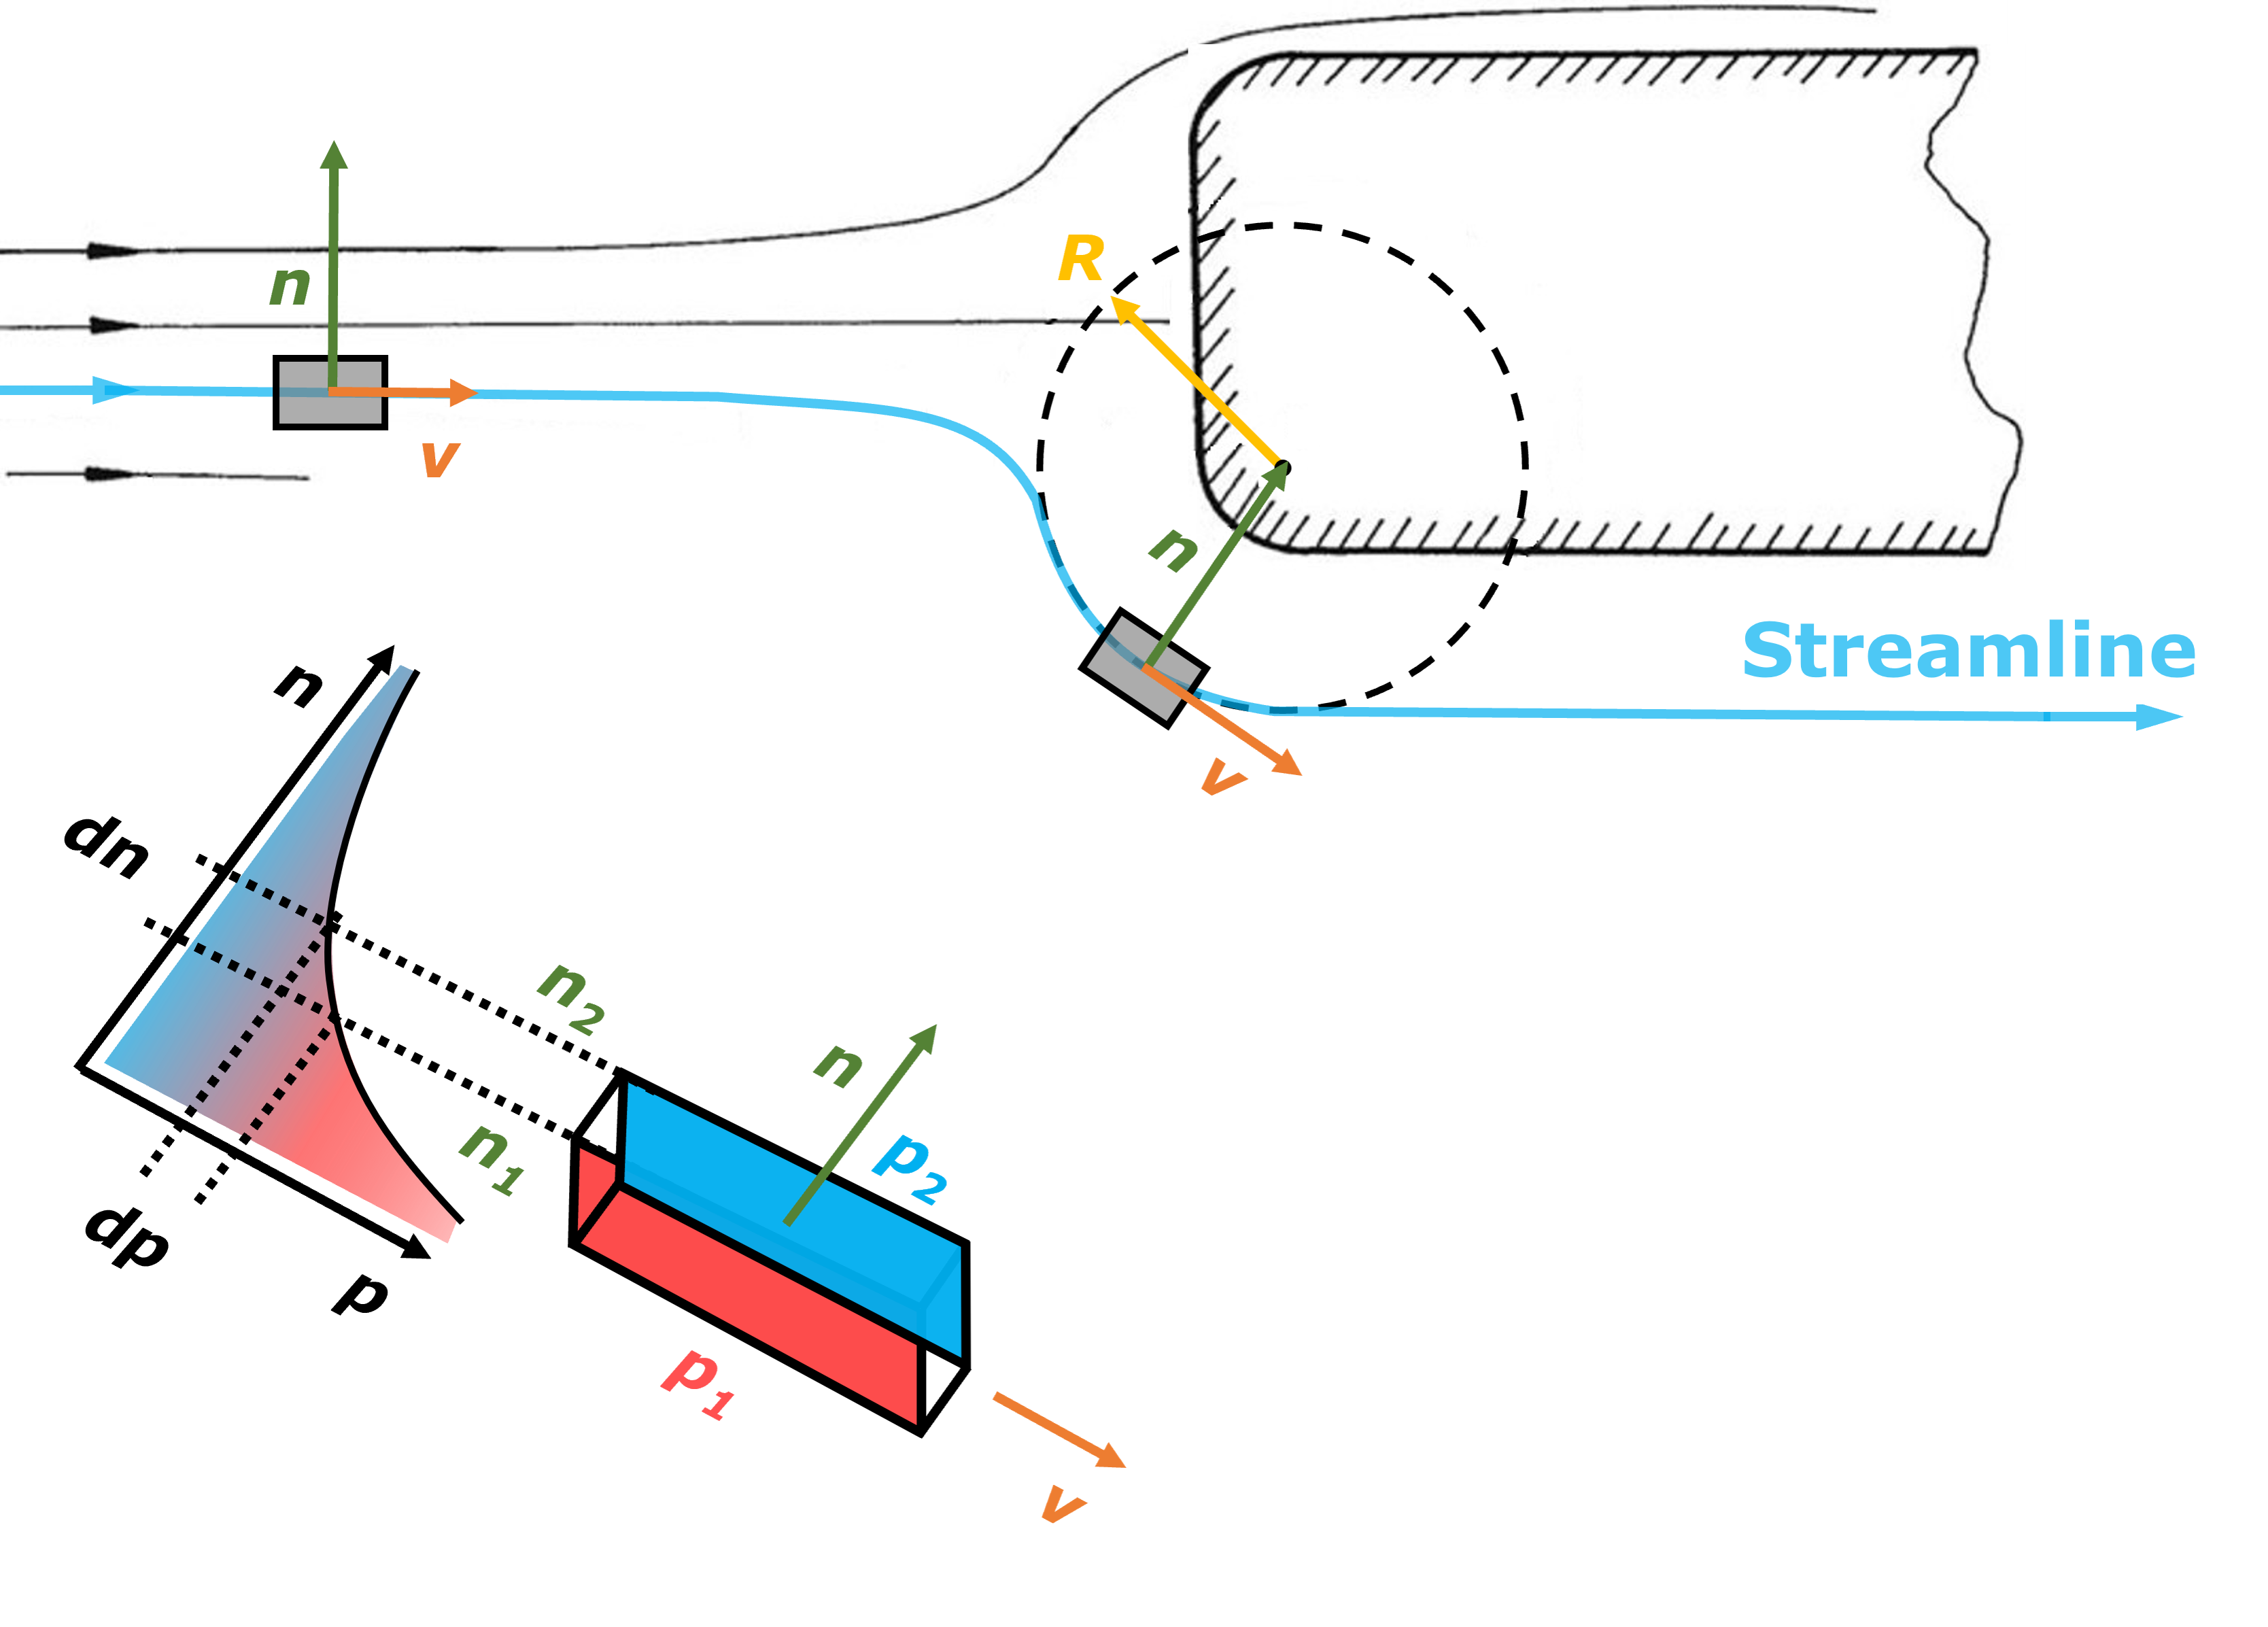
\includegraphics[width=\textwidth]{media/pressure_curvatur.png}
    \vspace*{-0.6cm}
    \begin{equation}
        \dfrac{dp}{dn} = -\rho\cdot\dfrac{v^2}{R}
    \end{equation}
\end{examplebox}

\vfill
\phantom{}
\columnbreak

\section{Mass conservation}
\subsection{Continuity equation / Mass conservation}
\begin{theorybox}{Continuity equation}
    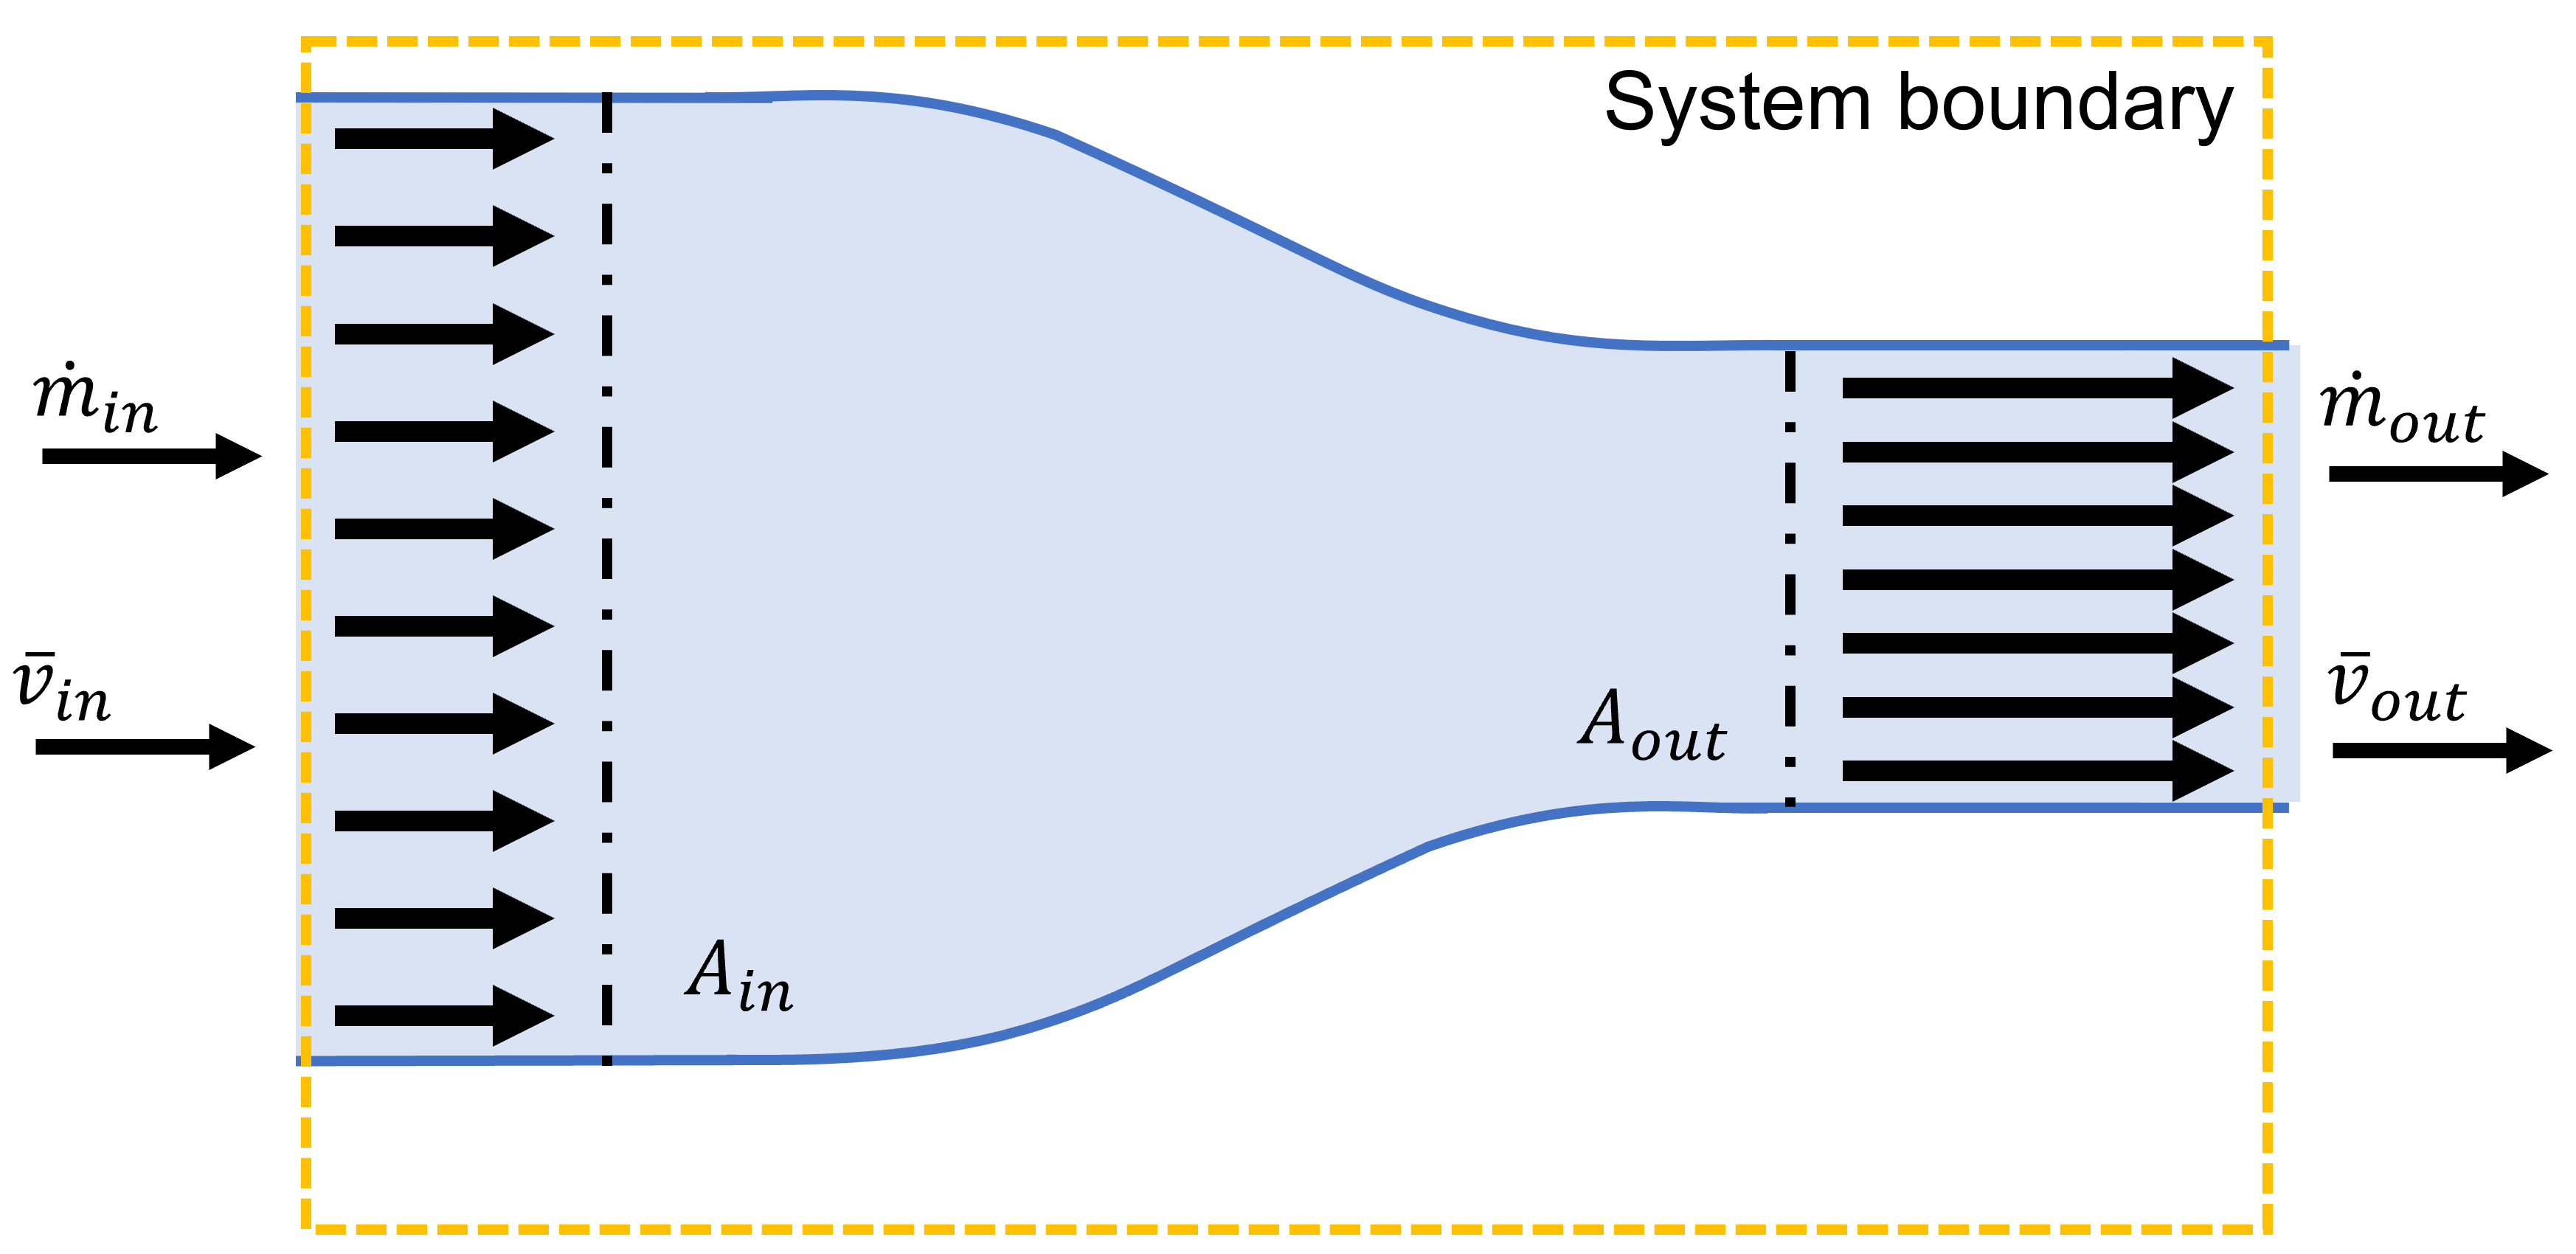
\includegraphics[width=\textwidth]{media/ContinuityBild1.png}
    \subsubsection{Steady mass-flow}
    \begin{equation}
    \dot m_{\rm in} = \dot m_{\rm out}
    \end{equation}

    \subsubsection{Incompressible fluid}
    \begin{equation}
    \dot m = \rho\,\dot V
    \quad\Longrightarrow\quad
    \dot V_{\rm in} = \dot V_{\rm out}
    \end{equation}

    \subsubsection{Streamline theory}
    \begin{equation}
    \dot V = \bar v\,A
    \quad\Longrightarrow\quad
    \bar v_{\rm in}\,A_{\rm in} = \bar v_{\rm out}\,A_{\rm out}
    \end{equation}
\end{theorybox}

\section{Energy conservation}
\subsection{Fluid mechanical energy conservation}
\begin{theorybox}{Derivation of the Bernoulli equation}
    \begin{equation}
        \dot{m}_1 \left(\dfrac{p_1}{\rho} + \dfrac{v_1^2}{2} + gz_1\right) = \dot{m}_2 \left(\dfrac{p_2}{\rho} + \dfrac{v_2^2}{2} + gz_2\right)
    \end{equation}
\subsubsection{Energy flow}
\vspace*{-0.5cm}
    \begin{align}
        \frac{dE}{dt} =\ 
        &\underbrace{\sum P + \sum \dot{Q}}_{
            \substack{
                \text{Energy flow} \\ \text{across system boundary}
            }
        } \notag \\
        &+ \underbrace{\sum_{in} \left[\dot{m}^{\swarrow} \cdot \left(h^{\swarrow} + \frac{v^{2\swarrow}}{2} + g z^{\swarrow}\right)\right]}_{
            \substack{
                \text{Energy transfer} \\ \text{mass in}
            }
        } \notag \\
        &- \underbrace{\sum_{out} \left[\dot{m}^{\nearrow} \cdot \left(h^{\nearrow} + \frac{v^{2\nearrow}}{2} + g z^{\nearrow}\right)\right]}_{
            \substack{
                \text{Energy transfer} \\ \text{mass out}
            }
        }
    \end{align}
\end{theorybox}



\vfill
\columnbreak
ciao

\end{multicols}
\end{document}